% Dataset section (Hiranya, issue #8)
% Needs: graphicx, booktabs, url (or hyperref). Figures are read from results/ (see \graphicspath in main.tex).

\section{Dataset}
\label{sec:dataset}

We use SROIE, the Scanned Receipts OCR and Information Extraction dataset of the ICDAR 2019 Robust Reading Challenge~\cite{huang2019sroie}. It contains scanned English-language receipts from Malaysia, and the key information extraction task (Task~3) asks for four fields per receipt: \emph{company}, \emph{date}, \emph{address} and \emph{total}. We use the standard split of 626 training and 347 test receipts.

\paragraph{Two versions of the same receipts.}
We combine two Hugging Face releases of SROIE, which contain the same receipt scans:
\begin{itemize}
  \item \texttt{darentang/sroie}\footnote{\url{https://huggingface.co/datasets/darentang/sroie}} provides, for every receipt, the OCR words, one bounding box per word already scaled to a $0$--$1000$ grid, and one BIO tag per word~\cite{ramshaw1995text}. With the label \texttt{O} and a \texttt{B-}/\texttt{I-} tag for each of the four fields, there are 9 labels. We use these tags to train BERT and LayoutLM and to build the main gold standard.
  \item \texttt{jsdnrs/ICDAR2019-SROIE}\footnote{\url{https://huggingface.co/datasets/jsdnrs/ICDAR2019-SROIE}} provides the receipt images and the official ICDAR answer strings for the four fields. It has no per-word tags. We use it for figures and for a second evaluation against the official answers.
\end{itemize}
The two are joined on the receipt key, the image file name (e.g.\ \texttt{X00016469612}). Every receipt in \texttt{darentang/sroie} has a match. The official test split contains 14 additional receipts that have no word tags; we leave them out so that all methods are evaluated on the same 347 test receipts. Figure~\ref{fig:receipt} shows a receipt with its word boxes coloured by label.

\begin{figure}[t]
  \centering
  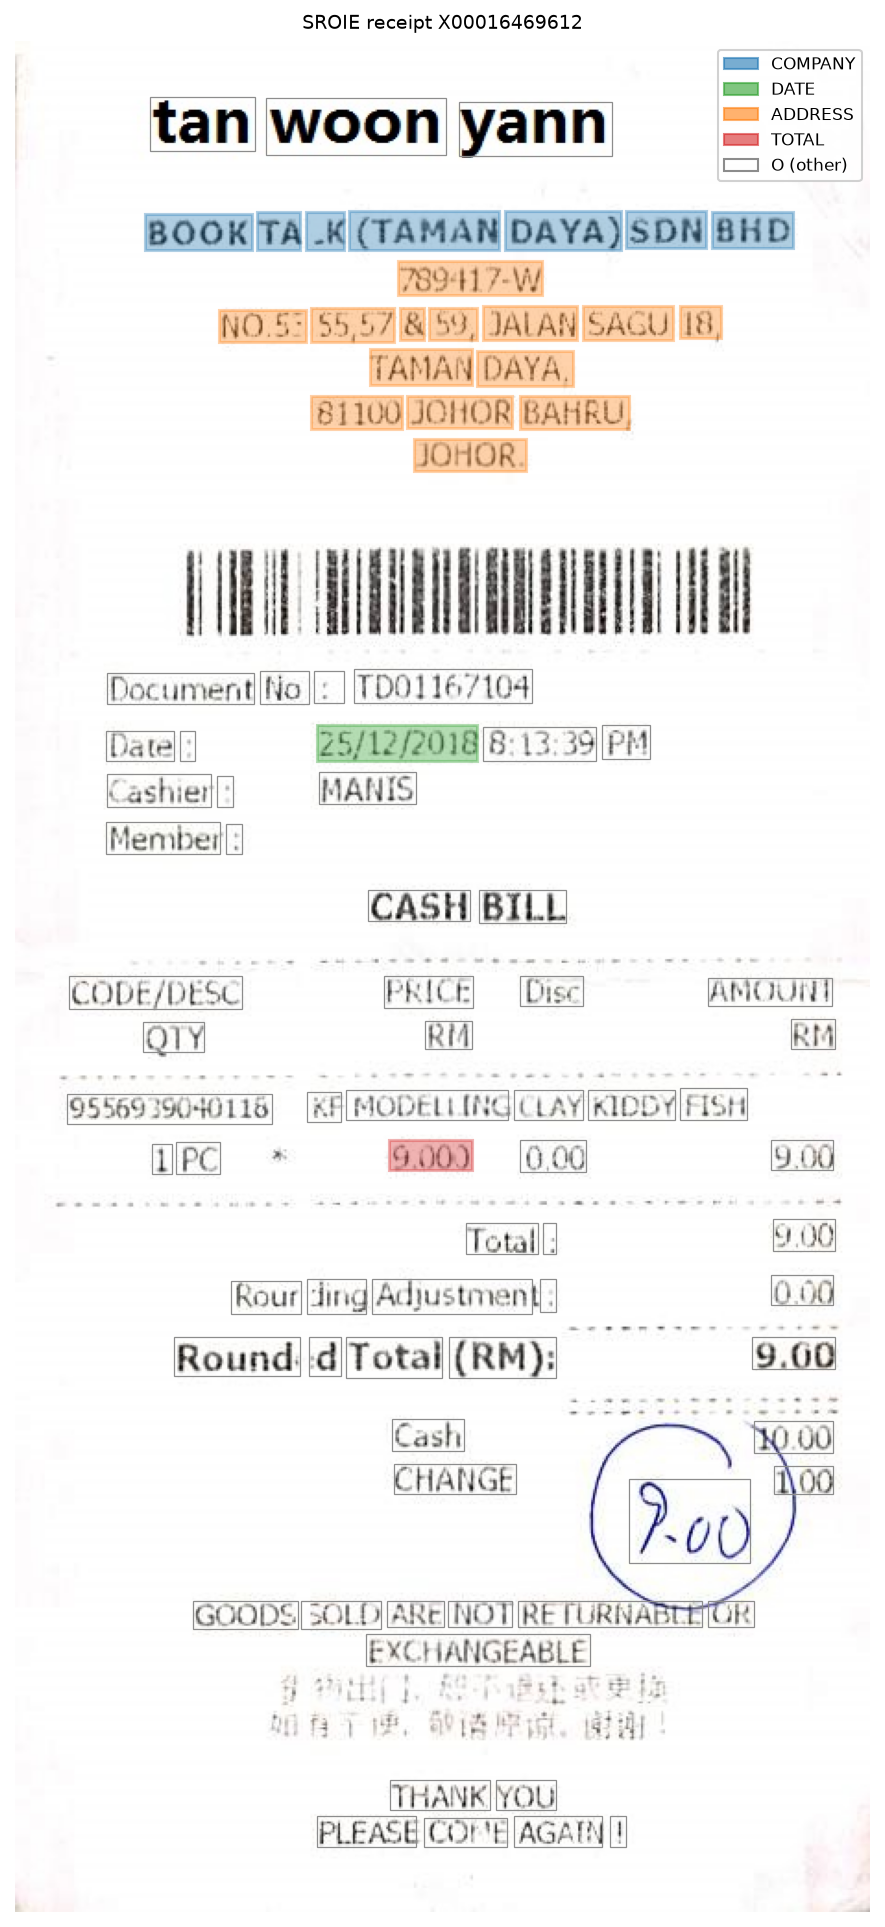
\includegraphics[width=0.36\linewidth]{receipt_example_1.png}
  \caption{A training receipt (\texttt{X00016469612}) with each OCR word box coloured by its tag: company (blue), address (orange), date (green), total (red), other (grey outline). The boxes are stored on a $0$--$1000$ grid and scaled back to pixels here; they line up with the printed words. The TOTAL tag sits on the item price \texttt{9.000} instead of the \texttt{9.00} on the total line (see Limitations).}
  \label{fig:receipt}
\end{figure}

\paragraph{Statistics.}
A receipt has $117.8$ OCR words on average in the training split ($116.5$ in the test split), ranging from 31 to 246. Most words are not part of any field: the label \texttt{O} covers $84.7\%$ of all words (Table~\ref{tab:labels} and Figure~\ref{fig:labels}). Every field is tagged exactly once per receipt as a single contiguous span, and all four fields are present in every receipt except one training receipt without an address. Address spans are the longest ($11.3$ words on average), company spans have $4.3$ words, and date and total are usually a single word.

\begin{table}[t]
  \centering
  \small
  \begin{tabular}{lrrr}
    \toprule
    Label & Train & Test & Share (\%) \\
    \midrule
    \texttt{O}         & 62{,}469 & 34{,}216 & 84.7 \\
    \texttt{B-COMPANY} &      626 &      347 &  0.9 \\
    \texttt{I-COMPANY} &  2{,}095 &  1{,}144 &  2.8 \\
    \texttt{B-DATE}    &      626 &      347 &  0.9 \\
    \texttt{I-DATE}    &      112 &       81 &  0.2 \\
    \texttt{B-ADDRESS} &      625 &      347 &  0.9 \\
    \texttt{I-ADDRESS} &  6{,}519 &  3{,}560 &  8.8 \\
    \texttt{B-TOTAL}   &      626 &      347 &  0.9 \\
    \texttt{I-TOTAL}   &       49 &       22 &  0.1 \\
    \midrule
    Receipts           &      626 &      347 &      \\
    Words              & 73{,}747 & 40{,}411 &      \\
    \bottomrule
  \end{tabular}
  \caption{Word-level label counts. The share is computed over both splits together.}
  \label{tab:labels}
\end{table}

\begin{figure}[t]
  \centering
  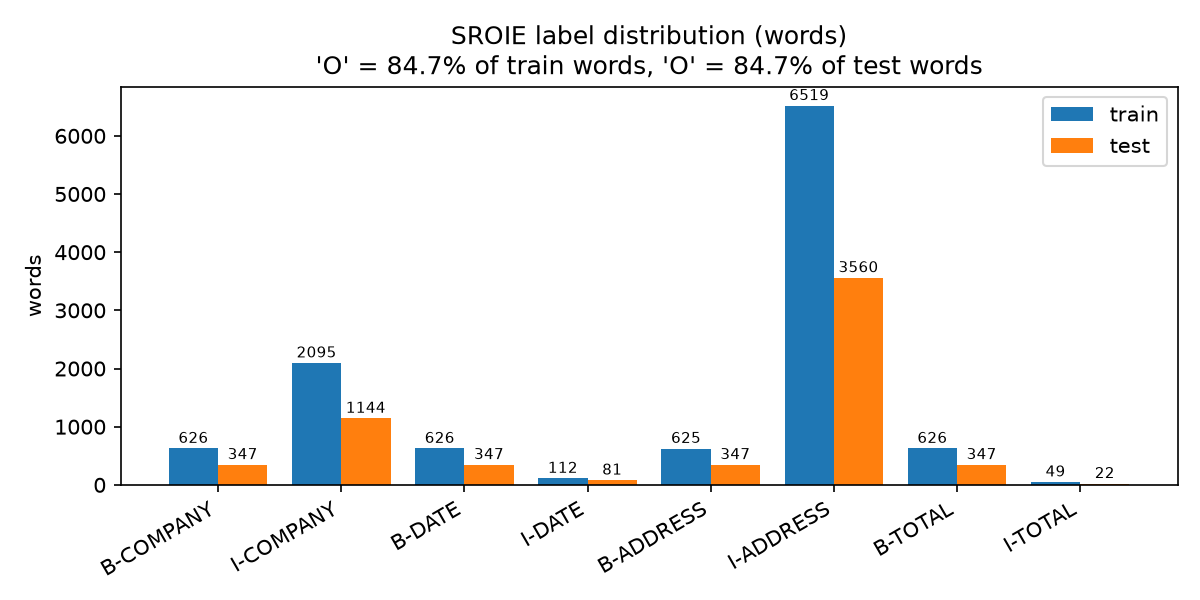
\includegraphics[width=0.7\linewidth]{label_distribution.png}
  \caption{Distribution of the field labels (words). \texttt{O}, not shown, makes up $84.7\%$ of all words.}
  \label{fig:labels}
\end{figure}

\paragraph{Sequence length.}
BERT and LayoutLM split words into WordPiece sub-tokens and read at most 512 of them. A receipt has about 257 sub-tokens on average ($2.2$ per word). Only 4 training receipts and 1 test receipt are longer than 512, and the words lost to truncation are never field words.

\paragraph{Limitations of the labels.}
The word tags were produced by matching the official answers against the OCR text, which leaves some noise:
\begin{itemize}
  \item \textbf{Total.} The total amount is usually printed several times (item price, subtotal, total line, cash), and $70\%$ of training receipts repeat its exact string. The tag is placed on the \emph{first} matching word in $96\%$ of the receipts, and only $67\%$ of TOTAL tags lie on a line that contains a word such as ``total'' or ``amount''. The layout cue ``the total is on the line that says TOTAL'' is therefore weaker in the labels than on the receipts.
  \item \textbf{Address and date.} Some address spans also include the company registration number (e.g.\ \texttt{789417-W} in Figure~\ref{fig:receipt}), and $2.6\%$ of date spans include extra words such as \texttt{Date:} or a time.
  \item \textbf{OCR noise.} The tagged words are OCR output, while the official answers were typed by annotators. Even a perfect tagger, scored against the official answers, would therefore not reach $100\%$ (Table~\ref{tab:ceiling}). The gap is largest for the address, where OCR spacing and misread characters (e.g.\ \texttt{SON BHD} for \texttt{SDN BHD}) break the exact match. For this reason our main evaluation uses the gold strings built from the word tags, and we report the official answers as a second score.
\end{itemize}

\begin{table}[t]
  \centering
  \small
  \begin{tabular}{lcc}
    \toprule
    Field & Exact match (\%) & Exact, ignoring spaces (\%) \\
    \midrule
    Company   & 80.4 & 80.7 \\
    Date      & 96.3 & 96.3 \\
    Address   & 58.2 & 74.4 \\
    Total     & 96.3 & 96.3 \\
    \midrule
    Macro avg & 82.8 & 86.9 \\
    \bottomrule
  \end{tabular}
  \caption{Upper bound for any tagging model scored against the official answers: the strings built from the gold word tags, compared with the official answers after the same normalisation as our evaluation (test split).}
  \label{tab:ceiling}
\end{table}
